\documentclass{article}

%============================================
%============================================
%===== PACKAGES AND DOCUMENT SETTINGS =====
%============================================
%============================================

%===== General margin setup =====
\setlength{\oddsidemargin}{0.25 in}
\setlength{\evensidemargin}{-0.25 in}
\setlength{\topmargin}{-0.6 in}
\setlength{\textwidth}{6.5 in}
\setlength{\textheight}{8.5 in}
\setlength{\headsep}{0.75 in}
\setlength{\parindent}{0 in}
\setlength{\parskip}{0.1 in}

%===== Packages that I normally like to use
\usepackage{amsmath,amssymb} %General math symbols and stuff
\usepackage[mathscr]{euscript} %To use script letters with \mathscr{}
\usepackage{amsthm} %To be able to write Definitions, Theorems, etc.
\usepackage{graphicx} % To scale equations and put figures wherever
\usepackage{framed} % To be able to frame theorems and stuff with begin{framed} ... \end{framed}
\usepackage{float} %To be able to place figures exactly where I want with [H]
\usepackage{multirow}
\usepackage{color}
\usepackage{cite}
\usepackage[hidelinks, breaklinks=true]{hyperref} %To be able to use links inside the document; [hidelinks removes the ugly red boxes]
\usepackage{xcolor}  \definecolor{shadecolor}{rgb}{.95,.95,.95}  %To put a shaded region
\usepackage[font=footnotesize]{caption}
\usepackage{nicefrac} %to put small fractions nicely with \nicefrac{1}{2}
\usepackage{ragged2e}	%to put \justify
\usepackage[shortlabels]{enumitem}	%To put letters in enumerate with begin{enumitem}[(a)]

%===== Algorithm setup =====
\usepackage[ruled,vlined]{algorithm2e}

%===== Example setup =====
\usepackage{mdframed}
\usepackage{changepage}
\newmdenv[
  topline=false,
  bottomline=false,
  skipabove=\topsep,
  skipbelow=\topsep
]{siderules}

%===== Theorems, lemmas, definitions, etc.
\theoremstyle{definition}
\newtheorem{myDefinition}{Definition}
\newtheorem{myTheorem}{Theorem}
\newtheorem{myLemma}{Lemma}
\newtheorem{myCorollary}{Corollary}
\newtheorem{myProposition}{Proposition}
\newtheorem{myExample}{Example}
\newtheorem{myExercise}{Exercise}
\newtheorem{myRemark}{Remark}
\newtheorem{myConjecture}{Conjecture}

%===== Page counters, theorem counters, etc.
\newcounter{lecnum}
\renewcommand{\thepage}{\thelecnum-\arabic{page}}
\renewcommand{\thesection}{\thelecnum.\arabic{section}}
\renewcommand{\theequation}{\thelecnum.\arabic{equation}}
\renewcommand{\thefigure}{\thelecnum.\arabic{figure}}
\renewcommand{\thetable}{\thelecnum.\arabic{table}}
\renewcommand{\themyDefinition}{\thelecnum.\arabic{myDefinition}}
\renewcommand{\themyTheorem}{\thelecnum.\arabic{myTheorem}}
\renewcommand{\themyLemma}{\thelecnum.\arabic{myLemma}}
\renewcommand{\themyCorollary}{\thelecnum.\arabic{myCorollary}}
\renewcommand{\themyProposition}{\thelecnum.\arabic{myProposition}}
\renewcommand{\themyExample}{\thelecnum.\arabic{myExample}}
\renewcommand{\themyExercise}{\thelecnum.\arabic{myExercise}}
\renewcommand{\themyRemark}{\thelecnum.\arabic{myRemark}}
\renewcommand{\themyConjecture}{\thelecnum.\arabic{myConjecture}}

%===== Header box =====
\newcommand{\lecture}[3]{
\pagestyle{myheadings}
\thispagestyle{plain}
\newpage
\setcounter{lecnum}{#1}
\setcounter{page}{1}
\noindent
\begin{center}
\rule{\textwidth}{1.6pt}\vspace*{-\baselineskip}\vspace*{2pt} % Thick horizontal line
\rule{\textwidth}{0.4pt}\\[1\baselineskip] % Thin horizontal line
\vbox{\vspace{2mm}
\hbox to 6.28in { {\bf CS 4980/6980: Introduction to Data Science} \hfill $\copyright$ Spring 2018 }
\vspace{4mm}
\hbox to 6.28in { {\Large \hfill Lecture #1: #2  \hfill} }
\vspace{4mm}
\hbox to 6.28in { {\scshape Instructor: Daniel L. Pimentel-Alarc\'on}  \hfill Scribed by: #3 }}
\vspace{-2mm}
\rule{\textwidth}{0.4pt}\vspace*{-\baselineskip}\vspace{3.2pt} % Thin horizontal line
\rule{\textwidth}{1.6pt}\\[\baselineskip] % Thick horizontal line
\end{center}
\markboth{Lecture #1: #2}{Lecture #1: #2}
\vspace*{4mm}
}

%====================================
%====================================
% ===== VARIABLES AND COMMANDS =====
%====================================
%====================================


%===== Some frequent commands that I use =====
\newcommand{\bs}[1]{\boldsymbol{#1}} %bold symbol
\newcommand{\hatt}[1]{\boldsymbol{\hat{#1}}} %bold hat
\newcommand{\careful}{\textcolor{red}}
\newcommand{\comment}{\textcolor{blue}}
\newcommand*\rot{\rotatebox{90}} %To rotate text in table
\newcommand*{\Scale}[2][4]{\scalebox{#1}{\ensuremath{#2}}} % To scale variables in equations

%===== In case you want to add colored text =====
\newcommand{\blue}{\textcolor{blue}}

%===== Miscelaneous math symbols =====
\def \R{\mathbb{R}}
\def \Pr{\mathsf{P}}
\def \T{\mathsf{T}}
\def \c{\mathsf{c}}
\def \spn{{\rm span}}
\def \Ord{\mathscr{O}}
\def \<{\langle}
\def \>{\rangle}
\DeclareMathOperator*{\argmin}{arg\,min}
\DeclareMathOperator*{\argmax}{arg\,max}

%===== Common scalars that will be used throughout =====
\def \D{{\hyperref[DDef]{{\rm D}}}} % ambient Dimension
\def \N{{\hyperref[NDef]{{\rm N}}}} %Number of samples
\def \xi{{\hyperref[xiDef]{{\rm x}}}} % a scalar variable x

%===== Common vectors that will be used throughout =====
\def \xx{{\hyperref[xxDef]{\bs{{\rm x}}}}} % a vector x
\def \yy{{\hyperref[yyDef]{\bs{{\rm y}}}}} % a vector y

%===== Common matrices that will be used throughout =====
\def \I{{\hyperref[IDef]{\bs{{\rm I}}}}} % Identity matrix
\def \X{{\hyperref[XDef]{\bs{{\rm X}}}}} % Data matrix

%Indices that will be used throughout.
\def \i{{\hyperref[iDef]{{\rm i}}}} % index used for samples, usually goes from 1 to N

%=====================================
%=====================================
%===== HERE BEGINS THE DOCUMENT =====
%=====================================
%=====================================

\begin{document}

%===== Lecture's number, title, and student's name.
\lecture{1} % Lecture number
{Lecture's title} % Lecture title
{YOUR NAME!} % Student's name

%===== Section
\section{Introduction}
This is how you include a figure:

\begin{figure}[h] %you can use [h], [b] or [t] to put the image "here", or at the "bottom" or at the "top".
\centering
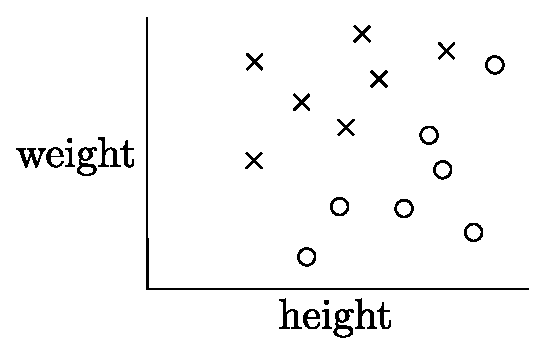
\includegraphics[width=5cm]{example_figure.eps}
\caption{This is how you put a caption.}
\label{nameFig}
\end{figure}

You can reference the figure as Figure \ref{nameFig}. You can also reference other things, like Table \ref{notationTab}.

\begin{table}[b]
\begin{center}
\begin{tabular}{| l | c | c c | c c | c c |}
\hline
& Examples & \rot{Regular } & \rot{Bold} & \rot{Lower} & \rot{Capital} & \rot{Roman} & \rot{Script} \\ \hline
Scalar & $\xi$ & $\checkmark$ & & $\checkmark$ & & $\checkmark$ & \\
$[$Column$]$ vector & $\xx$ & & $\checkmark$ & $\checkmark$  & & $\checkmark$  & \\
Matrix & $\X$ & & $\checkmark$ & & $\checkmark$ & $\checkmark$ & \\
Random variable & $x$ & $\checkmark$ & & $\checkmark$ & & & $\checkmark$ \\
Random vector & $\bs{x}$ & & $\checkmark$ & $\checkmark$  & & & $\checkmark$ \\
Random matrix & $\bs{X}$ & & $\checkmark$ & & $\checkmark$ & & $\checkmark$ \\ \hline
\end{tabular}
\caption{Throughout this course we will use standard mathematical notation.}
\label{notationTab}
\end{center}
\end{table}



Here is how you create an equation:
\begin{align*}
\xx_1 \ = \ \left[ \begin{matrix}
5'10" \\ 150 \\ 145
\end{matrix} \right]
%
\hspace{.5cm}
%
\xx_2 \ = \ \left[ \begin{matrix}
5'7" \\ 200 \\ 195
\end{matrix} \right]
%
\hspace{.5cm}
%
\xx_3 \ = \ \left[ \begin{matrix}
6'1" \\ 180 \\ 150
\end{matrix} \right]
%
\hspace{.5cm} \cdots \hspace{.5cm}
%
\xx_\N \ = \ \left[ \begin{matrix}
5'5" \\ 145 \\ 205
\end{matrix} \right]
\end{align*}

Here is how you create an ordered list:
\begin{enumerate}[(a)]
\item
List item \# 1.
\item
List item \# 2.
\item
List item \# 3.
\end{enumerate}

\begin{siderules}
\begin{myExample}[Example's title]
This is how an example should look (with two bars on the sides, to indicate beginning and end of the example. Putting tables and images in examples can be tricky. Here is how you put an image:

\center
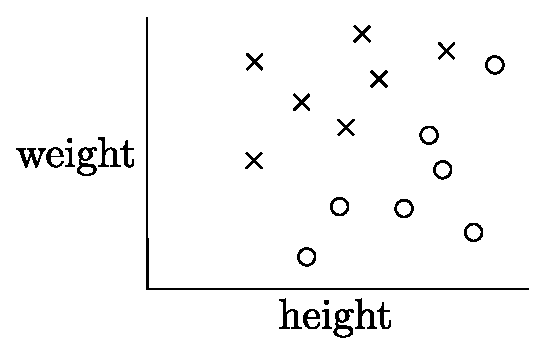
\includegraphics[width=5cm]{example_figure.eps}
\justify

Here is how you put a table:

\begin{center}
\begin{tabular}{| l || c | c | c | c | c |}
\hline
\textbf{Variables} & Individual 1 & Individual 2 & Individual 3 & $\cdots$ & Individual $\N$ \\ \hline \hline
Height & 5'10" & 5'7" & 6'1" & $\cdots$ & 5'5" \\ \hline
Weight & 150 & 200 & 180 & $\cdots$ & 145 \\ \hline
Glucose & 145 & 195 & 150 & $\cdots$ & 205 \\ \hline
\end{tabular}
\end{center}

\end{myExample}
\end{siderules}

\end{document} 



























